\chapter{Alcances y Limitaciones}
\label{chp:alcances}
Debido a la complejidad ....
\begin{itemize}
\item Actualmente no ...
\item Se limitará el número de danzas de interés a 4 (figura~\ref{fig:chp-alc:dance-dataset}), estas son: \textbf{Qhapac Chuncho, Qhapac Colla, Negrillos y Contradanza.}
\begin{figure}[!htb]
  \centering
  \caption{Danzas que serán usadas en el trabajo}
  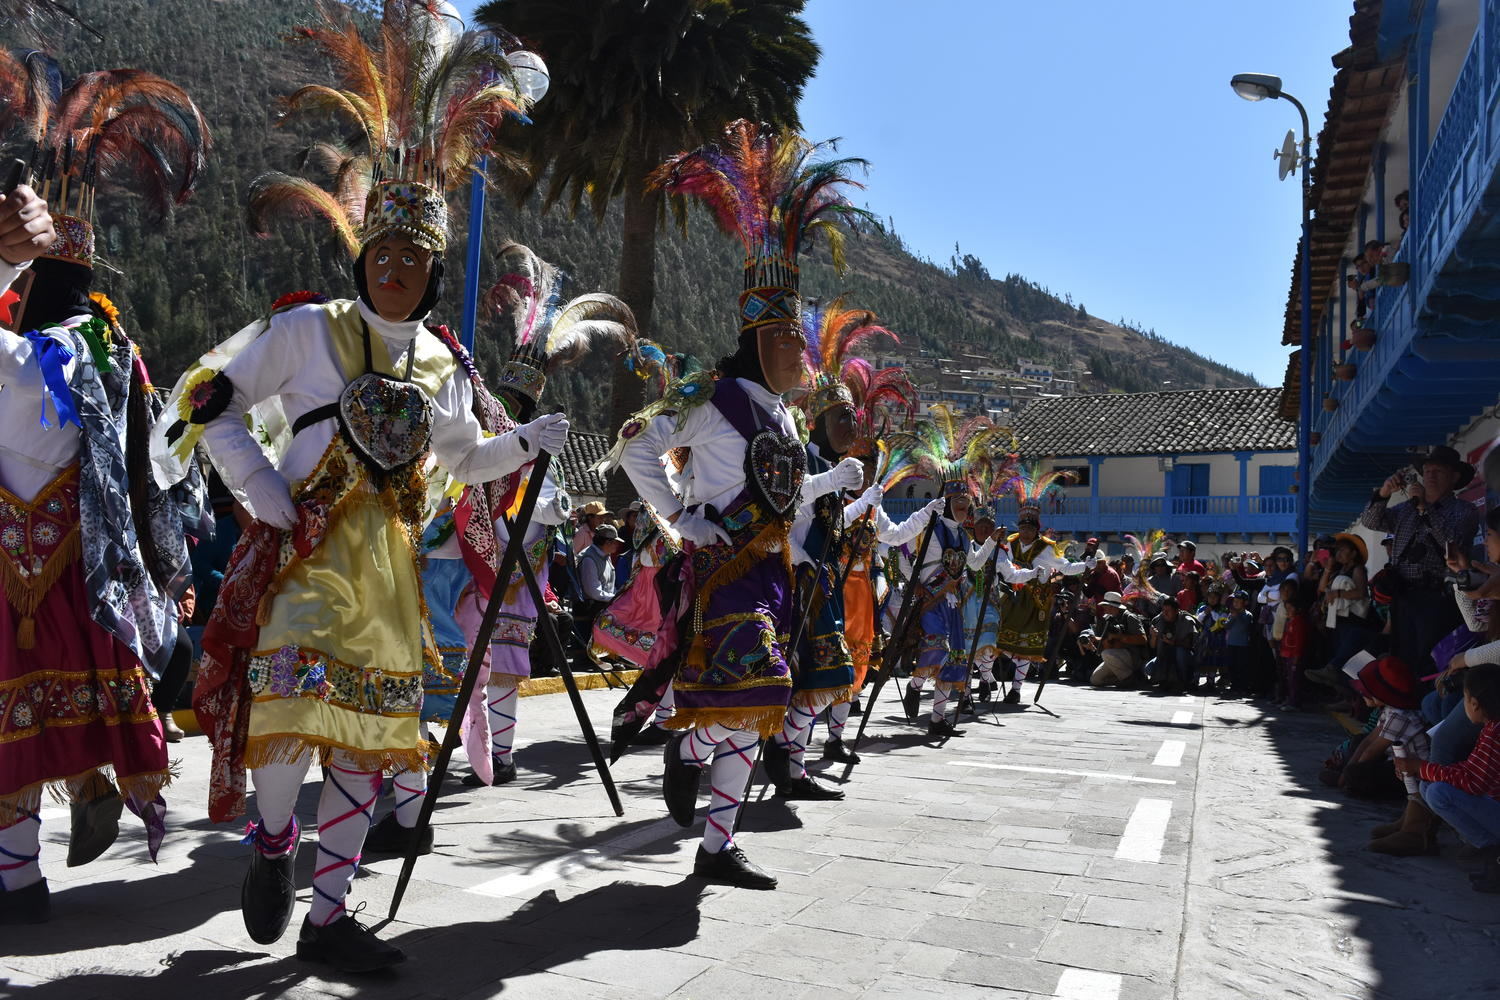
\includegraphics[width=0.4\textwidth]{figs/alcances/qhapacchuncho.JPG} \hspace*{0.01cm}
  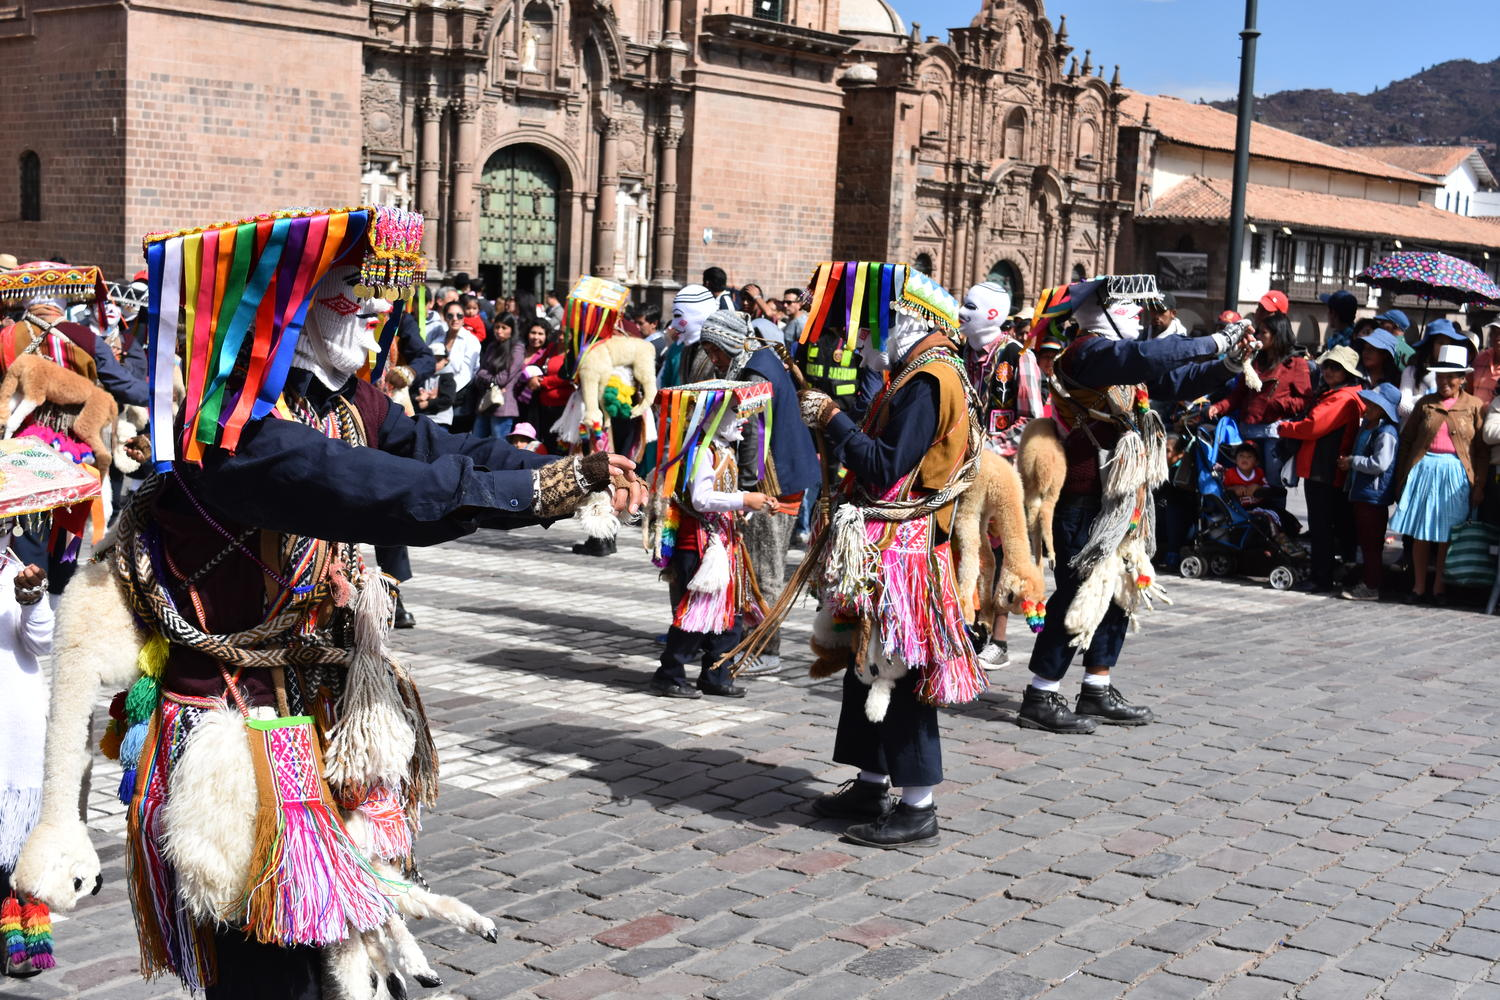
\includegraphics[width=0.4\textwidth]{figs/alcances/qhapaccolla.JPG} 
  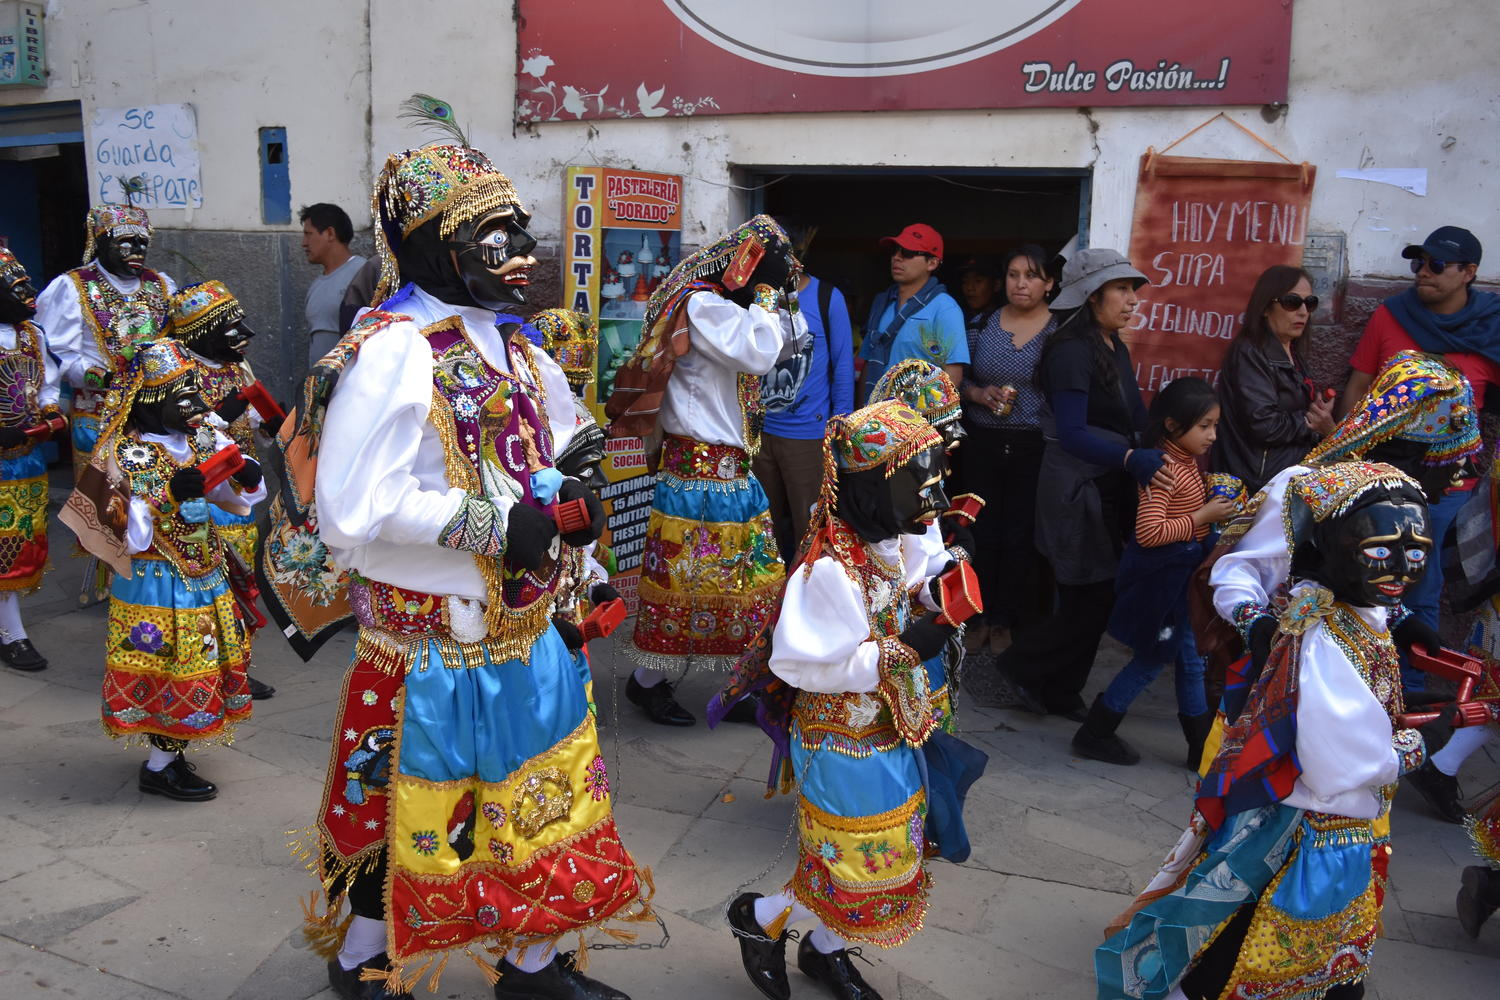
\includegraphics[width=0.404\textwidth]{figs/alcances/negrillo.JPG} \hspace*{0.01cm}
  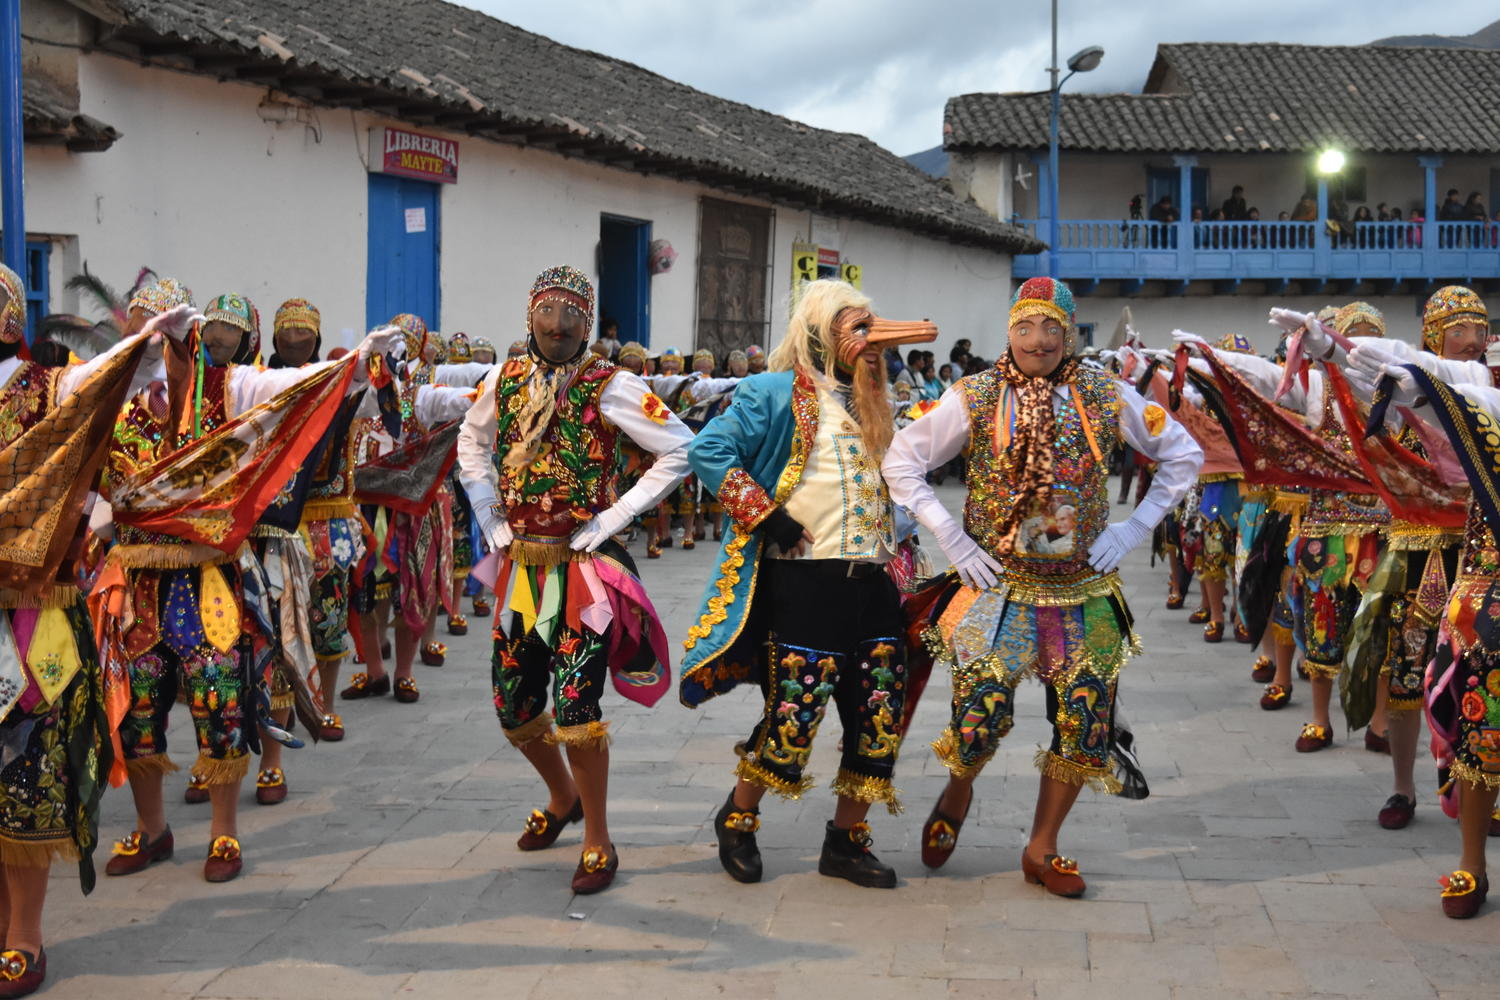
\includegraphics[width=0.4\textwidth]{figs/alcances/contradanza.JPG}
  \label{fig:chp-alc:dance-dataset}
\end{figure}

\item Para el procesamiento ...
\item Las técnicas que ...

\end{itemize}



